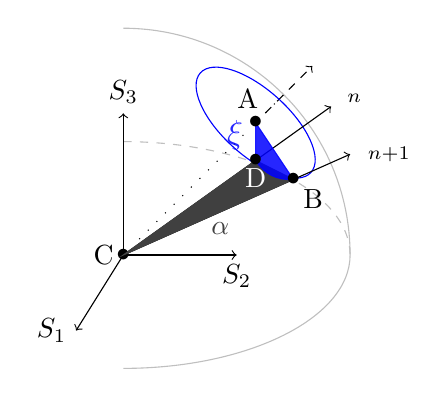
\begin{tikzpicture}[scale = 0.24]
    \node (C) at (0,0) {$\bullet$} node[left]{C};
    \node (A) at (7,7) {};
    \node (B) at (9,4) {};
    \node (D) at (7,5) {};

    \draw[lightgray, thin] (0,12) arc (90:0:12);
    \draw[lightgray, thin] (0,-6) arc (90:0:12cm and -6cm);
    \draw[lightgray, thin, dashed] (0,6) arc (90:0:12cm and 6cm);
    
    \draw[->] (C.center) --++ (0,7.5) node[above]{$S_3$};
    \draw[->] (C.center) --++ (6,0) node[below]{$S_2$};
    \draw[->] (C.center) --++ (-2.5,-4) node[left]{$S_1$};

    \draw[loosely dotted] (C) -- (A) --++ (2.25,2.25) node[right]{};
    \draw[->, dashed] (A) --++ (3,3) node[right, above]{$\vecu_{\vecS}$};
    %\draw[lightgray,dashed] (4.25,9.75) -- (9.75,4.25);
    \draw[lightgray, thin, rotate = 48, blue] (A) ellipse (1.75 and 3.9375);

    \draw[->] (C.center) --++ (12,5.33) node[xshift = 0.5cm, yshift = 0cm]{$\vecS_{n+1}$};
    \draw[->] (C.center) --++ (11,7.86) node[xshift = 0.3cm, yshift = 0.1cm]{$\vecS_{n}$};

    \filldraw[gray!50!black] (C.center) -- (B.center) node[midway, xshift = 0.15cm, , yshift = -0.15cm]{$\bm{\alpha}$} -- (D.center) -- cycle;
    \filldraw[blue, opacity = 0.85] (A.center) -- (B.center) node[midway, xshift = -0.5cm, yshift = 0.2cm]{\large $\bm{\xi}$} to[bend left] (D.center) -- cycle;

    \draw (A) node{$\bullet$} node[left of=A, xshift = 0.9cm, yshift = 0.3cm] {A};
    \draw (B) node{$\bullet$} node[xshift = 0.25cm, yshift = -0.25cm]{B};
    \draw (D) node{$\bullet$} node[left of=D, xshift = 1cm, yshift = -0.22cm, color = white] {D};
\end{tikzpicture}
